
\section{Dai numeri naturali ai numeri irrazionali}
\label{sec:radicali_irrazionali}
Nel volume Insiemi Numerici abbiamo presentato i diversi insiemi numerici. 
Li riprendiamo brevemente per poi approfondire i numeri reali e le loro 
proprietà.

L'insieme dei \emph{numeri naturali} racchiude i numeri che utilizziamo 
per contare; si indica nel seguente modo:
\[\N=\{0,1,2,3,4,5,6,7,8,9,10,11,\ldots\}\]

Su questi numeri sono definite le seguenti operazioni:
\begin{itemize*}
\item \emph{addizione}: \(n+m\) è il numero che si ottiene partendo da 
\(n\) e continuando a contare per altre \(m\) unità;
\item \emph{sottrazione}: \(n-m\) è il numero, se esiste, che 
addizionato a \(m\) dà come risultato \(n\);
\item \emph{moltiplicazione}: \(n \cdot m\) è il numero che si ottiene 
sommando 
\(n\) volte \(m\), o meglio sommando \(n\) addendi tutti uguali a \(m\)
\item \emph{divisione}: \(n:m\) è il numero, se esiste, che 
moltiplicato per \(m\) dà come risultato \(n\);
\item \emph{potenza}: \(n^{m}\) è il numero che si ottiene moltiplicando 
\(m\) 
fattori tutti uguali a \(n\) con \(m \ge 2\), ponendo \(n^{1}=n\) e 
\(n^{0}=1\);
\item \emph{radice}: \(\sqrt[{n}]{m}\) con \(n\ge 2\) è il numero, se 
esiste, 
che elevato a \(n\) dà come risultato \(m\).
\end{itemize*}

L'addizione, la moltiplicazione e la potenza sono definite su tutto 
l'insieme dei numeri naturali e sono operazioni interne a questo insieme,
cioè dati due numeri naturali qualsiasi, \(n\) 
ed \(m\), la somma \(n+m\) e il loro prodotto \(n \cdot m\) e la loro 
potenza \(n^{m}\), escluso il caso \(0^{0}\), danno come risultato un 
numero naturale. 
Non sempre invece, la differenza \(n-m\), il quoziente \(n:m\) o la 
radice \(\sqrt[{n}]{m}\) di due numeri naturali danno come risultato un 
numero naturale.

Tuttavia in molte situazioni vogliamo poter eseguire anche le sottrazioni, 
le divisioni e le radici e ottenere il risultato di queste operazioni 
anche se non è necessariamente un numero naturale. Per poter eseguire 
sempre le sottrazioni abbiamo inventato un nuovo insieme numerico: i 
numeri interi \(\Z\), per poter eseguire sempre (quasi) le divisioni 
abbiamo inventato i numeri razionali \(\Q\), per poter eseguire (almeno 
in certi casi) la radice, dovremo inventare un nuovo insieme numerico: 
l'insieme dei numeri reali \(\R\).

Con i numeri razionali, infatti, non è sempre possibile eseguire 
l'estrazione di radice. Consideriamo, ad esempio, \(\sqrt{2}\), cioè il 
numero che elevato al quadrato dà 2. La radice di due è un esempio 
particolarmente importante perché rappresenta la lunghezza della 
diagonale di un quadrato di lato uno.

\affiancati{.49}{.49}{
\immagine{Quadrato con diagonale posto su un asse x.}{\radicedidue}
}{
\immagine{Diagonale del quadrato riportata sull'asse x.}{\radicedidue}
}

La radice di due non è un numero razionale, cioè non può essere scritto 
né sotto forma di frazione né sotto forma di numero decimale finito o 
periodico. 
Supponiamo che la radice di due sia uguale a un numero razionale 
scritto come emme fratto enne con emme e enne \emph{primi fra di loro}: 
ad esempio 
\[\sqrt{2}=\dfrac{m}{n}\]
Se questo è vero, allora saranno vere anche le seguenti uguaglianze:
\[2= \dfrac{m^2}{n^2} \quad \text{ e } \quad 2n^2 = m^2\]
Questo vuol dire che \(m^2\) è un numero pari ma allora anche \(m\) deve 
essere pari quindi può essere scritto come il doppio di un altro numero:
\(m=2k\). sostituendolo nell'uguaglianza precedente otteniamo:
\[2n^2 = \tonda{2k}^2 \sRarrow 2n^2 = 4k^2 \sRarrow n^2 = 2k^2\]
Ma allora anche \(n^2\) è un numero pari. Quindi se la radice di due 
fosse esprimibile come rapporto tra due numeri, questi due numeri 
sarebbero contemporaneamente primi tra di loro e pari e quindi: supporre 
che \(\sqrt{2}\) sia un numero razionale porta a una contraddizione.


% Si può dimostrare che~\(\sqrt{2}\) non è un numero razionale con una 
% elegante dimostrazione per assurdo. 

% \begin{itemize*}
%  \item 
% Supponiamo che la radice di due sia un numero razionale scritto sotto 
% forma 
% di frazione~\(\sqrt{2}= \frac{a}{b}\), Certamente possiamo ridurre la 
% frazione 
% ai minimi termini.
%  \item 
% Se si elevano al quadrato entrambi i membri dell'equazione precedente, si 
% ottiene:~\(2=\frac{a^{2}}{b^{2}}\).
%  \item
% La precedente uguaglianza può anche essere scritta come \(2 \cdot b^2 = 
% a^2\), 
% da cui si deduce che \(a^2\) è un numero pari. Ma se \(a^2\) è pari lo 
% deve essere anche \(a\).
% quindi \(a\) può essere visto come il doppio di un 
% numero:~\(a=2 \cdot k\).
%  \item 
% L'uguaglianza precedente può essere vista come:~\(2 \cdot b^2 = (2 \cdot 
% k)^2\).
% Elevando al quadrato il monomio di destra si 
% ottiene:~\(2 \cdot b^2 = 4 \cdot k^2\).
%  \item 
% Dividendo per 2 entrambi i membri dell'uguaglianza 
% otteniamo:~\(b^2 = 2 \cdot k^2\). Da questo discende che anche~\(b^2\) 
% è pari e quindi anche \(b\), ma se sono entrambi pari allora la frazione 
% di partenza è riducibile contraddicendo che la frazione di partenza fosse 
% ridotta ai minimi termini.
% \end{itemize*}

% Elevare un numero al quadrato significa elevare al quadrato le
% singole potenze dei fattori primi in cui questo si scompone. 
% I fattori primi di~\(a^{2}\) e di~\(b^{2}\) sono gli stessi di~\(a\) e 
% di~\(b\) con gli esponenti raddoppiati, Se~\(a\) e~\(b\) non hanno 
% fattori in comune, anche~\(a^{2}\) e~\(b^{2}\) non li avranno. 
% Quindi ~\(a^{2}\) non può essere il doppio di~\(b^{2}\).
% Perciò~\(2\ne\frac{a^{2}}{b^{2}}\) e~\(\sqrt{2}\ne\frac{a}{b}\).
% 
% Oltre a \(\sqrt{2}\) vi sono altri infiniti numeri che non possono 
% essere scritti come frazione. 
% Molte radici e alcuni numeri particolari come \(\pi\), 
% che corrisponde alla misura della circonferenza di diametro \(1\).
% 
% Questi numeri sono detti \emph{numeri irrazionali} e costituiscono 
% l'insieme \(J\) dei numeri irrazionali.
% L'unione degli insiemi \(\Q\) e \(J\) è l'insieme \(R\) dei 
% numeri reali.



\begin{comment}
È possibile costruire l'insieme dei numeri reali a 
partire dall'insieme dei numeri razionali dividendoli in due insiemi~\(A\) 
e~\(B\) 
con particolari caratteristiche:
\begin{enumerate*}
\item \(A \cap B=\emptyset\)
\item \(A \cup B=\Q\)
\item \(\forall a \in A, \forall b \in B, a<b\)
\end{enumerate*}

Una coppia di insiemi con queste caratteristiche venne chiamato da 
Dedekind~(1831-1916) una \emph{sezione}, o \emph{partizione} di \(\Q\).

Dato che \(A\) e \(B\) devono avere intersezione nulla:

\begin{itemize*}
\item se \(A\) ha un massimo \(B\) non può avere un minimo;
\item se \(A\) non ha un massimo \(B\) può avere un minimo;
\item \(A\) può non avere un massimo \(B\) può non avere un minimo;
\end{itemize*}

% Nei primi due casi La sezione individua un numero Razionale, nel terzo 
% caso,
% individua un numero irrazionale.


\begin{esempio}{}{}
Sezioni
\begin{itemize}
\item I due insiemi \(A\) e \(B\) così definiti: 
\(A=\left\{x\in \Q |\, x<3\right\}\) e
\(B=\left\{x\in \Q |\, x \ge 3\right\}\) 
definiscono una sezione di \(\Q\), 
infatti \(A \cap B=\emptyset\) \(A \cup B=\Q\) e ogni elemento di A è 
minore 
di ogni elemento di B; 
inoltre possiamo osservare che \(A\) non ammette massimo,
non essendoci in esso un numero che sia maggiore di tutti gli altri, 
mentre \(B\) ammette il minimo che è 3;
\item siano \(A=\left\{x\in \Q |\, x<-1\right\}\), \(B=\left\{x \in \Q 
|\, 
x>0\right\}\) la coppia \((A,B)\) non è una sezione di \(\Q\) perché pur 
essendo 
\(A\cap B=\emptyset\) non è \(A\cup B=\Q\)
\item siano \(A=\left\{x\in \Q |\, x \le \frac{2}{7}\right\}\), 
\(B=\left\{x 
\in Q |\, x \ge \frac{2}{7}\right\}\), anche in questo caso la coppia 
\((A,B)\) 
non 
è una sezione di \(\Q\) poiché \(A\cap B=\left\{\frac{2}{7}\right\}\)
\item costruiamo gli insiemi \(A\) e \(B\) nel seguente modo: \(A\) sia 
l'unione 
tra 
l'insieme dei numeri razionali negativi e tutti i razionali il cui quadrato 
è 
minore di 2, in \(B\) mettiamo tutti i razionali il cui quadrato è maggiore 
di 
2. 
\(A=\Q^{-} \cup \left\{x \in \Q |\, x^{2}<2\right\}\), \(B=\left\{x \in 
\Q 
|\, x^{2}>2\right\}\). Si ha \(A \cap B=\emptyset\) \(A\cup B=\Q\), 
inoltre 
ogni 
elemento di \(A\) è minore di ogni elemento di \(B\), dunque \((A,B)\) è una 
sezione 
di \(\Q\), ma \(A\) non possiede il massimo e \(B\) non possiede il minimo, 
in 
quanto abbiamo già dimostrato che non esiste un numero razionale che ha \(2\) 
come 
quadrato. Questa sezione individua un buco nell'insieme \(\Q\).
\end{itemize}
\end{esempio}


\begin{definizione}{}{}
Si chiama \emph{elemento separatore} di una partizione \((A,B)\) di \(\Q\) 
il 
massimo di \(A\) o il minimo di \(B\), nel caso in cui almeno uno di questi 
elementi 
esista.
\end{definizione}

Nel primo esempio, poiché esiste il minimo di \(B\), la partizione \((A,B)\) 
ammette 
un elemento separatore e identifica il numero razionale \(3\).
Nel quarto esempio non esiste un numero razionale che fa da elemento 
separatore, 
la sezione \((A,B)\) identifica un numero irrazionale.

\begin{definizione}{}{}
L'insieme \(R\) dei numeri reali è l'insieme di tutte le partizioni di 
\(\Q\). Chiamiamo
numero razionale le partizioni che ammettono elemento separatore, chiamiamo 
\emph{numero irrazionale} le sezioni che non ammettono elemento separatore.
\end{definizione}

Ogni numero reale è individuato da due insiemi di numeri razionali che 
contengono, nel primo tutte le approssimazioni per difetto e il secondo
tutte le approssimazioni per eccesso.

% Ritornando all'esempio precedente, il numero \(\sqrt{2}\) è individuato 
% dalla 
% sezione costituita dagli insiemi \(A=\left\{x\in \Q |\, x<0\right\}\) 
% oppure 
% \(x^{2}<2\) e \(B=\left\{x\in \Q |\, x^{2}>2\right\}\).
% Nell'insieme \(A\) ci sono tutti i numeri razionali negativi oltre quelli 
% che 
% approssimano \(\sqrt{2}\) per difetto: 
% \[A=\{1;1,4;1,41;1,414;1,4142;1,414213;\ldots\}.\]
% Nell'insieme B ci sono tutti i numeri razionali che approssimano 
% \(\sqrt{2}\) 
% per eccesso:
% \[B=\{2;1,5;1,42;1,415;1,4143;1,41422;1,414214;\ldots\}.\]

Questa costruzione dell'insieme dei numeri reali \(R\) a partire 
dall'insieme dei numeri razionali \(\Q\) è puramente astratta e formale, 
non serve al calcolo, ma
permette di collegare i nuovi numeri all'insieme dei numeri naturali 
\(\N\). 

Nell'insieme delle partizioni di \(\Q\) è possibile definire in modo 
rigoroso 
l'ordinamento e le operazioni, nella pratica si usano sempre delle 
approssimazioni, magari molto elevate.

\begin{definizione}{}{}
Un insieme \(X\) si dice \emph{continuo} se ogni partizione \((X', X'')\) di 
\(X\) 
ammette uno e un solo elemento separatore, cioè se esiste un elemento \(x\) 
appartenente a \(X\) tale che per ogni \(x'\) di \(X'\) e per ogni \(x''\) 
di \(X''\) si ha \(x'{\leq}x{\leq}x''\).
\end{definizione}

\begin{teorema}{di Dedekind}
Ogni partizione dell'insieme \(R\) di numeri reali ammette uno e uno solo 
elemento separatore.
\end{teorema}

Da questo teorema segue che il numero reale è definito come l'elemento 
separatore di una sezione \((A,B)\) di numeri reali.

\end{comment}


% \subsection{Confronto fra numeri reali}
% Per confrontare due numeri reali, osserviamo prima di tutto i segni. Se i 
% segni dei numeri sono
% discordi, il numero negativo è minore del numero positivo. Se i segni dei 
% numeri sono concordi si valuta la parte intera del numero: se sono 
% positivi è 
% più grande quello che ha la parte intera maggiore, viceversa se sono 
% negativi 
% è più grande quello che ha la parte intera minore. A parità di parte 
% intera 
% bisogna confrontare la parte decimale partendo dalle cifre più a sinistra 
% finché non si 
% trova la prima cifra decimale diversa: se i numeri sono positivi è 
% maggiore 
% quello che ha la cifra maggiore; se sono negativi è maggiore quello che ha 
% la 
% cifra minore.
%
%  \begin{esempio}{}{}
%  Confrontare i seguenti numeri reali
%  \begin{itemize}
%  \item \(\sqrt{2}<\sqrt{3}\) per verificarlo ci si può aiutare con la 
% calcolatrice 
% per calcolare le prime cifre decimali dei due numeri 
% \(\sqrt{2}=1,4142\ldots\), 
% \(\sqrt{3}=1,7320\ldots\) oppure ci si arriva osservando che il numero che 
% elevato 
% al quadrato dà 2 deve essere minore del numero che elevato al quadrato dà 
% 3;
%  \item \(\sqrt{99}<10\) per verificarlo è sufficiente osservare che 
% \(\sqrt{100}=10\).
%  \end{itemize}
%  \end{esempio}
% 
% 
% \ovalbox{\risolvii \ref{ese:1.3}, \ref{ese:1.4}, \ref{ese:1.5}, 
% \ref{ese:1.6}, 
% \ref{ese:1.7}}\vspazio


% \begin{esempio}{}{}
%  \(f(x)=\valass{x-5}+\valass{x+2}\).
% 
%  La presenza di due valori assoluti ci obbliga a studiare i casi generati 
% dal 
% segno dei singoli argomenti.
%  Pertanto poiché l'argomento del primo valore assoluto è non negativo per 
% \(x\ge 
% 5\) e l'argomento del secondo valore assoluto è non negativo
%  per \(x\ge -2\), possiamo porre la reciproca situazione nel seguente 
% grafico:
% \begin{center}
% % (c) 2013 Claudio Carboncini - claudio.carboncini@gmail.com
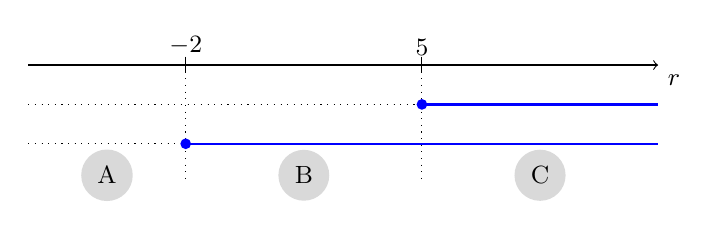
\begin{tikzpicture}[font=\small,x=10mm, y=10mm]

\draw[->] (0,0) -- (8,0) node [below right] () {$r$};

\foreach \x in {2,5}{
\draw(\x,3pt)--(\x,-3pt);
\begin{scope}[dotted]
\draw (\x,0) -- (\x,-1.5);
\draw (0,-.5) -- (5,-.5);
\draw (0,-1) -- (2,-1);
\end{scope}}

\node[above]  at (5,0) {$5$};
\node[above]  at (2,0) {$-2$};
\node [circle,fill=gray!30](A) at (1,-1.4) {A};
\node [circle,fill=gray!30](B) at (3.5,-1.4) {B};
\node [circle,fill=gray!30](C) at (6.5,-1.4) {C};

\begin{scope}[blue,thick]
\draw (5,-.5) -- (8,-.5);
\draw (2,-1) -- (8,-1);


\draw[fill=blue] (5,-.5)circle (1.5pt);
\draw[fill=blue] (2,-1)circle (1.5pt);

\end{scope}

\end{tikzpicture}

% \end{center}
% 
% \begin{enumerate}[label={(\Alph*)}]
%  \item \(x<-2\): in questo intervallo entrambi gli argomenti sono negativi, 
% pertanto 
% \[f(x)=\valass{x-5}+\valass{x+2}=-x+5-x-2=-2x+3.\]
% Se \(x=-2\) si ha \(f(-2)=\valass{-2-5}+0=7\)
%  \item \(-2<x<5\) il primo argomento è negativo e il secondo è positivo, 
% pertanto 
% \[f(x)=\valass{x-5}+\valass{x+2}=-x+5+x+2=7.\]
% Se \(x=5\) si ha \(f(5)=0+\valass{5+2}=7\)
%  \item \(x>5\) entrambi gli argomenti positivi, pertanto 
% \[f(x)=\valass{x-5}+\valass{x+2}=x-5+x+2=2x-3.\]
% \end{enumerate}
% Possiamo allora sintetizzare in questo modo
% \[
% \valass{x-5}+\valass{x+2}=\left\{\begin{array}{l}
% -2x+3 \text{, se }x<-2\\
% 7 \text{, se }-2\le x<5\\
% 2x-3 \text{, se }x\ge 5\end{array}.\right.
% \]
% \end{esempio}
% 
% \ovalbox{\risolvii \ref{ese:1.7}, \ref{ese:1.8}, \ref{ese:1.9}, 
% \ref{ese:1.10}, \ref{ese:1.11}}


\begin{comment}

\subsection{Radici quadrate}

\begin{definizione}{}{}
Si dice \emph{radice quadrata} di un numero reale positivo o nullo quel 
numero 
reale positivo o nullo che elevato al quadrato dà come risultato il numero 
dato.
In simboli~\(\sqrt a=b \Leftrightarrow b^2=a\) dove \(a,b\in \Rp \cup 
\{0\}\).
\end{definizione}

Il simbolo \(\sqrt{\quad}\) è il simbolo della radice quadrata; 
il numero \(a\) è detto \emph{radicando}, 
il numero \(b\) è detto \emph{radice quadrata} di \(a\).

Dalla definizione \(\sqrt{a^2}=a\) con \(a\ge 0\), quindi: 

\[\sqrt{81}=9 \text{ perché } 9^2=81 \quad 
\sqrt{\frac {9}{64}}=\frac{3}{8}
\text{ perché } \left(\frac 3 8\right)^2=\frac 9{64}\]

\osservazione \(\sqrt{81}=\sqrt{(-9)^2}\), ma non è vero che 
\(\sqrt{(-9)^2}=-9\) perché nella definizione di radice quadrata abbiamo 
imposto 
che il risultato dell'operazione di radice quadrata sia sempre un numero 
positivo o nullo.
Questa osservazione ci induce a porre molta attenzione quando il radicando è 
un'espressione letterale: in questo caso \(\sqrt{a^2}=a\) non è del tutto 
corretto poiché \(a\) può assumere sia valori positivi sia valori negativi
mentre, nei numeri reali, il risultato della radice quadrata non è mai un 
numero negativo. 
Scriveremo correttamente~\(\sqrt{a^2}=\valass{a}\).

% 
\begin{esempio}{}{}
Radici quadrate
\begin{htmulticols}{2}
\begin{itemize}
\item \(\sqrt 4=2\) infatti \(2^2=4\)
\item \(\sqrt{\dfrac 9{16}}=\dfrac 3 4\) infatti \(\left(\dfrac 3 4\right)^2=
\dfrac 9{16}\)
\item \(\sqrt{0,01}=0,1\) infatti \(0,1^2=0,01\)
\item \(\sqrt 1=1\) infatti \(1^2=1\)
\item \(\sqrt 0=0\) infatti \(0^2=0\)
\item \(\sqrt{-16}\) non esiste, radicando negativo;
\item \(\sqrt{11}\) esiste ma non è un numero intero né razionale, 
è un numero irrazionale;
\item \(\sqrt{x^2}=\left|x\right|\) dobbiamo mettere il valore assoluto 
al risultato perché non conoscendo il segno di \(x\) dobbiamo imporre che 
il risultato sia sicuramente positivo;
\item \(\sqrt{a^2-4a+4}=\sqrt{(a-2)^2}=\left|a-2\right|\) dobbiamo mettere 
il valore assoluto perché \(a-2\) può anche essere negativo;
\item \(\sqrt{9(x+1)^2}=3\left|x+1\right|\).
\end{itemize}
\end{htmulticols}
\end{esempio}
% 

\subsection{Radici cubiche}

\begin{definizione}{}{}
Si dice \emph{radice cubica} di un numero reale \(a\) quel numero che, 
elevato al cubo, dà come risultato \(a\). 
In simboli \(\sqrt[3]a=b \Leftrightarrow b^3=a\) dove \(a,b\in R\).
\end{definizione}

Puoi notare che la radice cubica di un numero reale esiste sempre sia per 
i numeri positivi o nulli, sia per i numeri negativi.

% 
\begin{esempio}{}{}
Radici cubiche
\begin{htmulticols}{2}
\begin{itemize}
\item \(\sqrt[3]{-8}=-2\) infatti \(\left(-2\right)^3=-8\)
\item \(\sqrt[3]{125}=5\) infatti \(5^3=125\)
\item \(\sqrt[3]1=1\) infatti \(1^3=1\)
\item \(\sqrt[3]0=0\) infatti \(0^3=0\)
\item \(\sqrt[3]{-1000}=-10\) infatti \(\left(-10\right)^3=-1000\)
\item \(\sqrt[3]{\dfrac 1 8}=\dfrac 1 2\) infatti 
\(\left(\dfrac 1 2\right)^3=\dfrac 1 8\)
\item \(\sqrt[3]{0,125}=0,5\) infatti \((0,5)^3=0,125\)
\item \(\sqrt[3]{x^3}=x\) per le radici cubiche non si deve mettere 
il valore assoluto;
\item \(\sqrt[3]{x^3+3x^2+3x+1}=\sqrt[3]{(x+1)^3}=x+1\) non si deve mettere 
il valore assoluto.
\end{itemize}
\end{htmulticols}
\end{esempio}
% 

Osserva che la radice cubica di un numero mantiene sempre lo stesso segno del 
numero in quanto il cubo di un numero reale conserva sempre il segno della 
base.

\subsection{Radici n-esime}
Oltre alle radici quadrate e cubiche si possono considerare radici di indice 
qualsiasi. 
Si parla in generale di radice \emph{n-esima} per indicare una radice con un 
qualsiasi indice \(n\).

\begin{definizione}{}{}
Si dice \emph{radice n-esima} di un numero reale~\(a\) quel numero~\(b\) che 
elevato alla~\(n\) dà come risultato~\(a\). Se~\(n\) è pari ~\(b\) è positivo.
In simboli~\(\sqrt[n]a=b \Leftrightarrow b^n=a\) con \(n\in \N, n > 0\).

\(a\) si dice \emph{radicando}, 

\(n\) si dice \emph{indice}, 

\(b\) si dice \emph{radice}

Non si definisce la radice di indice \(0\) e la scrittura \(\sqrt[0]a\) è 
priva 
di significato. Alla scrittura~\(\sqrt[1]a\) si dà il valore \(a\).
\end{definizione}

Quando si tratta con le radici n-esime di un numero reale, bisogna fare 
attenzione se l'indice della radice è pari o dispari. 
Si presentano infatti i seguenti casi:
\begin{itemize}
\item se l'indice \(n\) è dispari \(\sqrt[n]a\) è definita per qualsiasi 
valore 
di \(a\in R\), inoltre è negativa se~\(a<0\), positiva se \(a>0\) e 
nulla se \(a=0\)
\item se l'indice \(n\) è pari \(\sqrt[n]a\) è definita solo per i valori 
di~\(a\geq 0\) e si ha che \(\sqrt[n]a \ge 0\).
\end{itemize}

% 
\begin{esempio}{}{}
Radici n-esime
\begin{htmulticols}{2}
\begin{itemize}
\item \(\sqrt[4]{16}=2\) infatti \(2^4=16\)
\item \(\sqrt[4]{-16}\) non esiste infatti \((-2)^4=+16\)
\item \(\sqrt[5]{32}=2\) infatti \(2^5=16\)
\item \(\sqrt[4]1=1\) infatti \(1^4=1\)
\item \(\sqrt[n]0=0\)
\item \(\sqrt[5]{-1}=-1\) infatti \((-1)^5=-1\)
\item \(\sqrt[4]{x^4}=\left|x\right|\) va messo il valore assoluto perché 
  l'indice della radice è pari;
\item \(\sqrt[5]{x^5}=x\) non va messo il valore assoluto perché l'indice 
  della radice è dispari.
\end{itemize}
\end{htmulticols}
\end{esempio}
% 

% \ovalbox{\risolvii \ref{ese:2.1}, \ref{ese:2.2}, \ref{ese:2.3}, 
% \ref{ese:2.4},\ref{ese:2.5}, \ref{ese:2.6},\ref{ese:2.7}, 
% \ref{ese:2.8},\ref{ese:2.9}, \ref{ese:2.10}}

\section{Condizioni di esistenza}
\label{sec:radicali_condizioni_esistenza}

Riprendendo le conoscenze sulle potenze, ricordiamo che il quadrato di un 
numero non può essere negativo perché un numero negativo per se stesso dà 
come 
risultato un numero positivo. 
In generale una potenza con esponente pari è sempre positiva.  
Mentre una potenza con esponente dispari ha lo stesso segno della base.

\newpage

\begin{esempio}{}{}
Alcune potenze:

\begin{htmulticols}{4}
\((+5)^2=+25\)

\((-5)^2=+25\)

\((+2)^6=+64\)

\((-2)^6=+64\)

\((+2)^3=+8\)

\((-2)^3=-8\)

\((+2)^7=+128\)

\((-2)^7=-128\)
\end{htmulticols}

\end{esempio}

Possiamo affermare che nessun numero reale può essere la radice quadrata di 
un numero negativo, poiché non esiste nessun numero reale che elevato al 
quadrato dia come risultato un numero negativo. 

E, più in generale, nessun numero reale può essere la radice di indice pari 
di un numero negativo.

Finché abbiamo a che fare con numeri, le cose risultano abbastanza semplici, 
ma quando il radicando è un'espressione letterale dobbiamo fare molta 
attenzione a operare su di esso.

Non è detto che \(sqrt{a}\) esista, perché non possiamo sapere se~\(a\) 
rappresenta un numero positivo o negativo. 
Quindi \(sqrt{a}\) è un numero reale solo se~\(a \ge 0\).

Le \emph{condizioni di esistenza} (in breve si può scrivere \(\CE\)) 
di un radicale sono le condizioni cui devono 
soddisfare le variabili che compaiono nel radicando affinché la radice 
sia un numero reale.

Supponiamo di avere \(\sqrt[n]{A(x)}\) con \(A(x)\) espressione nella
variabile~\(x\), dobbiamo distinguere i seguenti casi:
\begin{itemize*}
\item se \(n\) è pari la radice è un numero reale solo per i valori 
di~\(x\) che rendono non negativo il radicando, cioè \(\CE: A(x)\ge 0\)
\item se \(n\) è dispari la radice è un numero reale per qualsiasi valore 
della variabile~\(x\) che permette di calcolare il radicando.
\end{itemize*}

% 
\begin{esempio}{}{}
Condizioni di esistenza
\begin{itemize}
\item \(\sqrt x\):\quad \(\CE x\ge 0\)
\item \(\sqrt[3]x\):\quad \(\CE \forall x\in R\)
\item \(\sqrt{-x}\):\quad \(\CE x\le 0\)
\item \(\sqrt[3]{-x}\):\quad \(\CE \forall x\in R\)
\item \(\sqrt{x-1}\):\quad \(\CE x-1\ge 0 \Rightarrow x\ge 1\)
\item \(\sqrt{a^2+1}\):\quad \(\CE \forall a\in R\), infatti \(a^2\) è 
sempre 
  positivo pertanto \(a^2+1>0, \forall a\in R\)
\item \(\sqrt[3]{\frac 1{x+1}}\):\quad la radice cubica è definita per 
valori 
  sia positivi sia negativi del radicando, tuttavia bisogna comunque porre 
la 
  condizione che il denominatore della frazione non sia nullo, 
  quindi \(\CE x+1\neq 0 \Rightarrow x\neq -1\)
\item \(\sqrt[4]{xy}\):\quad \(\CE xy\ge 0\)
\item \(\sqrt[5]{a^2(a-3)}\): poiché la radice ha indice dispari non occorre 
  porre alcuna condizione di esistenza.
\end{itemize}
\end{esempio}

\begin{esempio}{}{}
Determina le condizioni di esistenza della seguente 
espressione: \(\sqrt x+\sqrt{x+1}\).

C.E. \(\sqrt x\) esiste per \(x\ge 0\), \(\sqrt{x+1}\) 
esiste per \(x+1\ge 0\), quindi per individuare le condizioni di esistenza 
dell'espressione occorre risolvere il sistema 
\(\left\{\begin{array}{l} x\ge0\\ x+1\ge0\end{array}\right.
\Rightarrow\left\{\begin{array}{l}x\ge0\\x\ge-1\end{array}\right.\).

\begin{center}
% (c) 2013 Claudio Carboncini - claudio.carboncini@gmail.com
\begin{tikzpicture}[font=\small,x=10mm, y=10mm]

\draw[->] (0,0) -- (8,0) node [below right] () {$r$};

\foreach \x in {2,5}{
\draw(\x,3pt)--(\x,-3pt);
\begin{scope}[dotted]
\draw (\x,0) -- (\x,-1.5);
\draw (0,-.5) -- (2,-.5);
\draw (0,-1) -- (5,-1);
\end{scope}}

\node[above]  at (2,0) {$-1$};
\node[above]  at (5,0) {$0$};
\pattern[pattern= north east lines, pattern color=red] (5,-1) rectangle (8,-1.5);

\node[below] () at (6.5,-1.5) {$\IS$};

\begin{scope}[blue,thick]
\draw (2,-.5) -- (8,-.5);
\draw (5,-1) -- (8,-1);

\draw[fill=blue] (2,-.5)circle (1.5pt);
\draw[fill=blue] (5,-1)circle (1.5pt);

\end{scope}

\end{tikzpicture}

\end{center}

In definitiva \(\CE x\ge 0\).
\end{esempio}

\begin{esempio}{}{}
Determina le condizioni di esistenza della radice 
\(\sqrt[4]{\dfrac{x-1}{x+1}}\).

C.E. \(\dfrac{x-1}{x+1}\ge 0\). 
Occorre discutere il segno della frazione \(f\), combinando il segno del 
numeratore \(N\) e del denominatore \(D\):

\begin{center}
% (c) 2013 Claudio Carboncini - claudio.carboncini@gmail.com
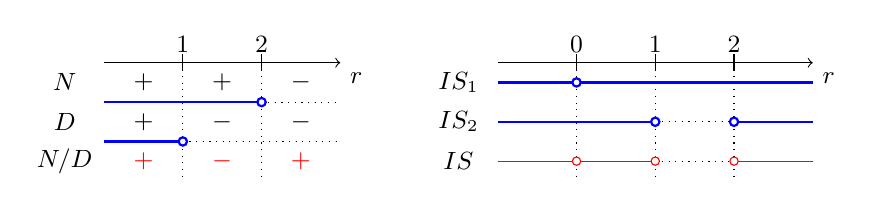
\begin{tikzpicture}[font=\small,x=10mm, y=10mm]

\draw[->] (0,0) -- (3,0) node [below right] () {$r$};
\draw[->] (5,0) -- (9,0) node [below right] () {$r$};

\foreach \x in {1,2,6,7,8}{
\draw(\x,3pt)--(\x,-3pt);
\begin{scope}[dotted]
\draw (\x,0) -- (\x,-1.5);
\draw (2,-.5) -- (3,-.5);
\draw (1,-1) -- (3,-1);
\draw (7,-.75) -- (8,-.75);
\draw (7,-1.25) -- (8,-1.25);
\end{scope}}

\node[above]  at (1,0) {$1$};
\node[above]  at (2,0) {$2$};
\node[above]  at (6,0) {$0$};
\node[above]  at (7,0) {$1$};
\node[above]  at (8,0) {$2$};

\begin{scope}[blue,thick]
\draw (0,-.5) -- (2,-.5);
\draw (1,-1) -- (0,-1);
\draw (5,-.25) -- (6,-.25);
\draw (5,-.25) -- (9,-.25);
\draw (5,-.75) -- (7,-.75);
\draw (8,-.75) -- (9,-.75);

\draw[fill=white] (2,-.5)circle (1.5pt);
\draw[fill=white] (1,-1)circle (1.5pt);
\draw[fill=white] (6,-.25)circle (1.5pt);
\draw[fill=white] (7,-.75)circle (1.5pt);
\draw[fill=white] (8,-.75)circle (1.5pt);
\end{scope}

\foreach \x in {4.5}{
\node  at (\x,-.25) {$IS_1$};
\node  at (\x,-.75) {$IS_2$};
\node  at (\x,-1.25) {$IS$};
}
\foreach \x in {-0.5}{
\node  at (\x,-.25) {$N$};
\node  at (\x,-.75) {$D$};
\node  at (\x,-1.25) {$N/D$};
}

\foreach \z in {.5,1.5}
\node  at (\z,-.25) {$+$};

\foreach \zi in {1.5,2.5}
\node  at (\zi,-.75) {$-$};

\node  at (2.5,-.25) {$-$};
\node  at (0.5,-.75) {$+$};

\begin{scope}[red]
\foreach \y in {-1.25}{
\foreach \ziv in {1.5}
	\node at (\ziv,\y) {$-$};
\foreach \zv in {.5,2.5}
\node at (\zv,\y) {$+$};
\draw (5,-1.25) -- (7,-1.25);
\draw (8,-1.25) -- (9,-1.25);
\draw[fill=white] (6,-1.25)circle (1.5pt);
\draw[fill=white] (7,-1.25)circle (1.5pt);
\draw[fill=white] (8,-1.25)circle (1.5pt);

}
\end{scope}
\end{tikzpicture}

\end{center}
Pertanto C.E. \(x<-1\vee x\ge 1\).
\end{esempio}
% 

% \vspazio\ovalbox{\risolvii \ref{ese:2.11}, \ref{ese:2.12}, \ref{ese:2.13}, 
% \ref{ese:2.14},\ref{ese:2.15}}

\end{comment}


\begin{comment}

In questo paragrafo ci proponiamo di scrivere la radice n-esima di un 
numero 
reale \(a\geq0\) sotto forma di potenza di \(a\), vogliamo cioè che sia:
\(\sqrt[n]a=a^x\).

\paragraph {Caso con esponente positivo}
Elevando ambo i membri dell'uguaglianza alla potenza~\(n\) otteniamo: 
\(\left(\sqrt[n]a\right)^n=\left(a^x\right)^n\) da cui si ottiene 
\(a=a^{n\cdot x}\).
Trattandosi di due potenze con base~\(a{\geq}0\), l'uguaglianza è resa 
possibile 
solo se sono uguali gli esponenti. 
In altre parole, deve essere: \(1=n\cdot x \Rightarrow x=\dfrac 1 n\), 
quindi: \(\sqrt[n]a=a^{\frac 1 n}\).

Vediamo ora di generalizzare la formula. Sia \(m\) un numero intero positivo, 
possiamo scrivere \(a^{\frac m n}=\left(a^{\frac 1 n}\right)^m\) e 
quindi \(a^{\frac m n}=\left(\sqrt[n]a\right)^m\).

% 
\begin{esempio}{}{}
Calcola le seguenti potenze a esponente razionale positivo.
\begin{itemize*}
\item~\(27^{\frac{2}{3}}\): si ha che 
  \(27^{\frac{2}{3}}=\left(\sqrt[3]{27}\right)^2=3^2=9\)
\item~\(25^{\frac 3 2}\): si ha che 
  \(25^{\frac 3 2}=\left(\sqrt[2]{25}\right)^3=5^3=125\).
\end{itemize*}
\end{esempio}
% 

\paragraph{Caso con esponente negativo}
Per definire la potenza ad esponente razionale negativo è necessario 
imporre 
la restrizione \(a{\neq}0\), infatti risulta:
\(a^{-\frac m n}=\dfrac 1{a^{\frac m n}}=\left(\dfrac 1 a\right)^{\frac m n}\)

% 
\begin{esempio}{}{}
Calcola le seguenti potenze a esponente razionale negativo.
\begin{itemize*}
\item \(27^{-\frac{2}{3}}=\dfrac 1{\left(\sqrt[3]{27}\right)^2}=
  \dfrac 1{3^2}=\dfrac 1 9\)
\item \(125^{-\frac{2}{3}}=\sqrt[3]{125^{-2}}=\sqrt[3]{(5^3)^{-2}}=
  \sqrt[3]{(5^{-2})^3}=5^{-2}=\dfrac 1{25}\)
\item \(\left(\dfrac 1 8\right)^{-\frac 3 2}=
  \sqrt{\left(\dfrac 1 8\right)^{-3}}=\sqrt{8^3}=\sqrt{(2^3)^3}=\sqrt{2^9}\)
\item \(\left(\dfrac 1{49}\right)^{-\frac 1 2}=(49)^{\frac 1 2}=\sqrt{49}=7\)
\end{itemize*}
\end{esempio}
% 

In generale si dà la seguente
\begin{definizione}{}{}
Si dice \emph{potenza a esponente razionale} \(\frac m n\) di un numero reale 
positivo \(a\) l'espressione:
\(a^{\frac m n}=\sqrt[n]{a^m}=\left(\sqrt[n]a\right)^m\) con 
\(\frac m n\in \Q\).
\end{definizione}

Perché abbiamo dovuto imporre la condizione che~\(a\) sia un numero positivo?
Partiamo dall'espressione \(a^{\frac 1 n}\) con \(n\in \N-\{0\}\), 
se \(n\) è dispari la potenza \(a^{\frac 1 n}\) è sempre definita per ogni 
valore 
della base \(a\), mentre se è pari \(a^{\frac 1 n}\) è definita solo 
per \(a{\geq}0\).

Nel caso generale \(a^{\frac m n}\) con \(\frac m n\in \Q\) 
la formula \(a^{\frac m n}=\left(\sqrt[n]a\right)^m\) è falsa se \(a<0\).

Consideriamo il seguente esempio:
\((-2)^{\frac 6 6}=\left[(-2)^{\frac 1 
6}\right]^6=\left(\sqrt[6]{-2}\right)^6\) 
non è definita nei numeri reali perché non esiste la radice sesta di un 
numero 
negativo.
Tuttavia possiamo anche scrivere 

\[(-2)^{\frac 6 6}=\left[(-2)^6\right]^{\frac 1 6}=(64)^{\frac 1 6}=
\sqrt[6]{64}=2.\]

Arriviamo pertanto a due risultati differenti.

Per estendere la definizione al caso di basi negative sarebbe necessario 
stabilire un ordine di priorità delle operazioni ma ciò andrebbe contro la 
proprietà commutativa del prodotto degli esponenti di una potenza di 
potenza.

% \vspazio\ovalbox{\risolvii \ref{ese:2.16}, \ref{ese:2.17}, 
\ref{ese:2.18}, 
% \ref{ese:2.19},\ref{ese:2.20}}

\end{comment}


% \newpage
% % 
%  \begin{esempio}{}{}
%  Radici equivalenti.
%  \begin{itemize}
%  \item \(\sqrt{2}=\sqrt[4]{2^2}\) abbiamo moltiplicato per \(2\) indice 
% della radice ed esponente del radicando;
%  \item \(\sqrt[3]a=\sqrt[9]{a^3}\) abbiamo moltiplicato per \(3\) indice 
% della radice ed esponente del radicando.
% \end{itemize}
%  \end{esempio}
% % 
% 
% \begin{teorema}{}{}
% Il valore di una radice in \(Rp \cup \{0\}\) non cambia se dividiamo 
% l'indice della radice e l'esponente del radicando per un loro divisore 
% comune. 
% In simboli \(\sqrt[nt]{a^{mt}}=\sqrt[n]{a^m}\) con \(a\ge 0\) e 
% \(m,n,t\in \N-\{0\}\).
% \end{teorema}


% Per rendersi conto di questa proprietà si possono trasformare le radici 
% in 
% potenze ad esponenti razionali e applicare le proprietà delle potenze:
%  \[\sqrt[n]a\cdot \sqrt[n]b=a^{\frac 1 n}\cdot b^{\frac 1 n}=(ab)^{\frac 
% 1 
% n}=
%    \sqrt[n]{ab},\quad \sqrt[n]a:\sqrt[n]b=a^{\frac 1 n}:b^{\frac 1 n}=
%    \left(\dfrac a b\right)^{\frac 1 n}=\sqrt[n]{\dfrac a b}.\]


% \paragraph{I° modo:} si esegue la divisione intera \(m:n\) ottenendo un 
% quoziente \(q\) e un resto \(r\). Per la proprietà della divisione si 
% ha \(m=n\cdot q+r\) quindi \(\sqrt[n]{a^m}=\sqrt[n]{a^{n\cdot q+r}}\) 
% e per le proprietà delle potenze 
% \(\sqrt[n]{a^{n\cdot q+r}}=\sqrt[n]{(a^q)^n\cdot a^r}\) 
% e per la regola del prodotto di due radici con medesimo indice si ottiene:
% 
% \[\sqrt[n]{a^{n\cdot q+r}}= \sqrt[n]{(a^q)^n\cdot a^r}=
%   \sqrt[n]{(a^q)^n}\cdot \sqrt[n]{a^r}=
%   a^q\cdot \sqrt[n]{a^r}\text{ con } r<n.\]
% Notiamo che il fattore ``fuori`` dalla radice ha per esponente il quoziente 
% della divisione intera, mentre il fattore che rimane ``dentro`` ha per 
% esponente il resto della divisione stessa.
% 
%  \(\sqrt[3]{a^8}=\ldots \) eseguiamo la divisione \(8:3\) con \(q=2\) e 
% \(r=2\), 
%  otteniamo \(\sqrt[3]{a^8}=a^2\cdot \sqrt[3]{a^2}\).

% \paragraph{II° modo:} 


% \begin{osservazione}{}{}
% Quanto scritto sopra sembra filare, ma c'è un problema: \emph{il segno}:
% % .
% % Osserviamo i seguenti passaggi:
% \[\tonda{-3} \cdot \sqrt{5} = \sqrt{\tonda{-3}^2 \cdot 5} = 
%   \sqrt{9 \cdot 5} = +3 \cdot \sqrt{5}\]
% Se dividiamo la prima e l'ultima espressione 
% per \(\sqrt{5}\) otteniamo: \(-3 = +3\) e questo non è accettabile.
% Questo problema sorge quando l'indice della radice è un numero pari.
% \end{osservazione}


% % \newpage
% % 
%  \begin{esempio}{}{}
%  Potenza di radice.
%  \begin{htmulticols}{2}
%  \begin{itemize}
%  \item \(\left(\sqrt{2}\right)^2=\sqrt{2^2}=2\)
%  \item \(\left(\sqrt[3]{2ab^2c^3}\right)^2=\sqrt[3]{4a^2b^4c^6}\).
%  \end{itemize}
%  \end{htmulticols}
%  \end{esempio}


% Le espressioni con radicali possono essere trasformate in potenze con 
% esponente frazionario per poi applicare le proprietà delle potenze:
% 
% % 
% Trasforma i radicali in potenze con esponente frazionario applicando le 
% proprietà delle potenze.
%  \begin{esempio}{}{}
% % \begin{itemize}
% %  \item
%   \[\dfrac{\sqrt a\cdot \sqrt[3]{a^2\cdot b}}{\sqrt[6]{a^5\cdot b}}=
%    \dfrac{a^{\frac 1 2}\cdot a^{\frac{2}{3}}\cdot 
%           b^{\frac 1 3}}{a^{\frac 5 6}\cdot b^{\frac 1 6}}=
%    a^{\frac 1 2+\frac{2}{3}-\frac 5 6}\cdot b^{\frac 1 3-\frac 1 6}=
%    a^{\frac 2 6}\cdot b^{\frac 1 6}=\sqrt[6]{a^2b}\]
%  \end{esempio}
%  \begin{esempio}{}{}
% %  \item
% %   \(\sqrt{\dfrac{\sqrt[3]{a^2}\cdot \sqrt b}{\sqrt[5]{a^2}}}\cdot 
% %    \sqrt[3]{\dfrac{\sqrt[4]{a^6b}}{a\sqrt[3]b}}\).
%  \begin{align*}
%  \sqrt{\frac{\sqrt[3]{a^2}\cdot \sqrt b}{\sqrt[5]{a^2}}}\cdot
%  \sqrt[3]{\frac{\sqrt[4]{a^6b}}{a\sqrt[3]b}}&=
%  \left(\frac{a^{\frac{2}{3}}\cdot b^{\frac 1 2}}
%  {a^{\frac 2 5}}\right)^{\frac 1 2}\left(\frac{a^{\frac 3 2}\cdot 
%   b^{\frac 1 4}}{ab^{\frac 1 3}}\right)^{\frac 1 3}\\ &=
%   \frac{a^{\frac 1 3}\cdot b^{\frac 1 4}}{a^{\frac 1 5}}\cdot 
%   \frac{a^{\frac 1 2}\cdot b^{\frac 1{12}}}{a^{\frac 1 3}\cdot b^{\frac 1 
% 9}}\\
%  &=a^{\frac 1 3-\frac 1 5\;+\frac 1 2-\frac 1 3}\cdot 
%    b^{\frac 1 4+\frac 1{12}-\frac 1 9}\\
%  &=a^{\frac 3{10}}\cdot b^{\frac 2 9}\\
%  &=\sqrt[10]{a^3}\cdot \sqrt[9]{b^2};
%  \end{align*}
%  \end{esempio}
% %  \begin{esempio}{}{}
% % %  \item 
% % %    \(\sqrt[6]{\dfrac{x^3\cdot \sqrt[3]{xy^2}}{x^2-\sqrt{xy}}}\)
% %  \begin{align*}
% %  \sqrt[6]{\frac{x^3\cdot \sqrt[3]{xy^2}}{x^2-\sqrt{xy}}}&=
% %  \left(\frac{x^3\cdot (xy^2)^{\frac 1 3}}{x^2-(xy)^{\frac 1 2}}\right)^
% %    {\frac 1 6}\\
% %  &=\left(\frac{x^3\cdot x^{\frac 1 3}\cdot y^{\frac{2}{3}}}
% %               {x^2-x^{\frac 1 2}\cdot y^{\frac 1 2}}\right)^{\frac 1 
% 6}\\
% %  &=\left(\frac{x^{\frac{10} 3}\cdot y^{\frac{2}{3}}}
% %               {x^{\frac 1 2}\cdot \left(x^{\frac 3 2}-y^{\frac 1 
% 2}\right)}
% %               \right)^{\frac 1 6}\\
% %  &=\left[x^{\frac{17} 6}\cdot y^{\frac{2}{3}}\cdot
% %    \left(x^{\frac 3 2}-y^{\frac 1 2}\right)^{-1}\right]^{\frac 1 6}\\
% %  &=x^{\frac{17}{36}}\cdot y^{\frac 1 9}\cdot 
% %       \left(x^{\frac 3 2}-y^{\frac 1 2}\right)^{-\frac 1 6}.
% %  \end{align*}
% % % \end{itemize}
% %  \end{esempio}
% % 
% \vspazio\ovalbox{\risolvii \ref{ese:2.50}, \ref{ese:2.51}, 
% \ref{ese:2.52}, 
% \ref{ese:2.53}, \ref{ese:2.54}, \ref{ese:2.55}, \ref{ese:2.56}, 
% \ref{ese:2.57}, \ref{ese:2.58}, \ref{ese:2.59}, \ref{ese:2.60}, 
% \ref{ese:2.61}, \ref{ese:2.62},}
% 
% \vspazio\ovalbox{\ref{ese:2.63}, \ref{ese:2.64}, \ref{ese:2.65}, 
% \ref{ese:2.66}, \ref{ese:2.67}}


% \paragraph{IV° Caso:}
% la frazione è del tipo \(\dfrac x{\sqrt a+\sqrt b+\sqrt c}\)
% 
% Anche in questo caso si utilizza il prodotto notevole della differenza di 
% quadrati, solo che va ripetuto più volte.
% 
% % 
%  \begin{esempio}{}{}
% Razionalizza \(\dfrac 1{\sqrt{2}+\sqrt{3}+\sqrt 5}\).
% 
% Il fattore di razionalizzazione è in questo caso \(\sqrt{2}+\sqrt{3}-\sqrt 
% 5\) 
% quindi:
%  \[\dfrac 1{\sqrt{2}+\sqrt{3}+\sqrt 5}\cdot 
%    \dfrac{\sqrt{2}+\sqrt{3}-\sqrt 5}{\sqrt{2}+\sqrt{3}-\sqrt 5}=
%    \dfrac{\sqrt{2}+\sqrt{3}-\sqrt 5}{(\sqrt{2}+\sqrt{3})^2-5}=
%    \dfrac{\sqrt{2}+\sqrt{3}-\sqrt 5}{2+3+2\sqrt 6-5}=
%    \dfrac{\sqrt{2}+\sqrt{3}-\sqrt 5}{2\sqrt 6};\]
%  ora il fattore razionalizzante di questa frazione è \(\sqrt 6\):
%  \[\dfrac{\sqrt{2}+\sqrt{3}-\sqrt 5}{2\sqrt 6}\cdot \dfrac{\sqrt 6}{\sqrt 
% 6}=
%  \dfrac{\sqrt{12}+\sqrt{18}-\sqrt{30}}{2\cdot 6}=
%  \dfrac{2\sqrt{3}+3\sqrt{2}-\sqrt{30}}{12}.\]
%  \end{esempio}
% % 
% 
% \paragraph{V° Caso:} 
% la frazione è del tipo \(\dfrac x{\sqrt[3]a+\sqrt[3]b}\).
% 
% In questo caso si utilizza il prodotto notevole 
% \((a+b)(a^2-ab+b^2)=a^3+b^3\) e quello analogo~\((a-b)(a^2+ab+b^2)=a^3-b^3\).
% \begin{align*}
% \frac x{\sqrt[3]a+\sqrt[3]b}=
% \frac x{\sqrt[3]a+\sqrt[3]b}\cdot 
% \frac{\sqrt[3]{a^2}-\sqrt[3]{ab}+\sqrt[3]{b^2}}
%      {\sqrt[3]{a^2}-\sqrt[3]{ab}+\sqrt[3]{b^2}}=&
%      \frac{x\left(\sqrt[3]{a^2}-\sqrt[3]{ab}+\sqrt[3]{b^2}\right)}
%           {(\sqrt[3]a)^3+(\sqrt[3]b)^3}\\
% &=\frac{x\left(\sqrt[3]{a^2}-\sqrt[3]{ab}+\sqrt[3]{b^2}\right)}{a+b}.
% \end{align*}
% 
% % 
%  \begin{esempio}{}{}
% Razionalizza \(\dfrac 1{\sqrt[3]{2}-\sqrt[3]{3}}\).
% 
% Il fattore di razionalizzazione è in questo caso 
% \(\sqrt[3]{2^2}+\sqrt[3]{2\cdot 3}+\sqrt[3]{3^2}\) quindi:
%  \[\dfrac{1\cdot \left(\sqrt[3]{2^2}+\sqrt[3]{2\cdot 
% 3}+\sqrt[3]{3^2}\right)}
%          {\left(\sqrt[3]2-\sqrt[3]3\right)\cdot \left(\sqrt[3]{2^2}+
%           \sqrt[3]{2\cdot 3}+\sqrt[3]{3^2}\right)}=
%    \dfrac{\sqrt[3]{2^2}+\sqrt[3]{2\cdot 3}+\sqrt[3]{3^2}}{2-3}=
%    -\left(\sqrt[3]4+\sqrt[3]6+\sqrt[3]9\right).\]
%  \end{esempio}
% % 
% \vspazio\ovalbox{\risolvii \ref{ese:2.68}, \ref{ese:2.69}, 
% \ref{ese:2.70}, 
% \ref{ese:2.71}, \ref{ese:2.72}, \ref{ese:2.73}, \ref{ese:2.74}, 
% \ref{ese:2.75}, \ref{ese:2.76}}

% \section{Radicali doppi}
% \label{sec:radicali_radicali_doppi}
% 
% Si dice radicale doppio un'espressione del tipo \(\sqrt{a+\sqrt b}\) 
% oppure \(\sqrt{a-\sqrt b}\).
% 
% I radicali doppi possono essere trasformati nella somma algebrica di due 
% radicali semplici se l'espressione \(a^2-b\) è un quadrato perfetto. 
% La formula per ottenere la trasformazione in radicali semplici è:
% 
% \begin{equation*}
% \sqrt{a\pm \sqrt b}=
% \sqrt{\dfrac{a+\sqrt{a^2-b}} 2}\pm \sqrt{\dfrac{a-\sqrt{a^2-b}} 2}
% \end{equation*}
% 
% % 
%  \begin{esempio}{}{}
% Trasforma, se possibile, i seguenti radicali doppi in radicali semplici.
% \begin{itemize}
%  \item \(\sqrt{7-\sqrt{40}}=
%  \sqrt{\dfrac{7+\sqrt{49-40}} 2}-\sqrt{\dfrac{7-\sqrt{49-40}} 2}=
%  \sqrt{\dfrac{7+3} 2}-\sqrt{\dfrac{7-3} 2}=\sqrt 5-\sqrt{2}\)
%  \item \(\sqrt{2-\sqrt{3}}=
%  \sqrt{\dfrac{2+\sqrt{2^2-3}} 2}-\sqrt{\dfrac{2-\sqrt{2^2-3}} 2}=
%  \sqrt{\dfrac 3 2}-\sqrt{\dfrac 1 
% 2}=\dfrac{\sqrt{3}-\sqrt{2}}{\sqrt{2}}\), 
%  razionalizzando il denominatore si ottiene: 
%  \(\dfrac{\sqrt{3}-\sqrt{2}}{\sqrt{2}}=
%  \dfrac{(\sqrt{3}-\sqrt{2})\cdot \sqrt{2}}{\sqrt{2}\cdot \sqrt{2}}=
%  \dfrac{\sqrt 6-\sqrt{2}} 2\)
%  \item \(\sqrt{7+2\sqrt 6}=\sqrt{7+\sqrt{24}}\)
%  per applicare la formula abbiamo portato il fattore \(2\) dentro la 
% radice: 
%  \(\sqrt{7+\sqrt{24}}=
%  \sqrt{\dfrac{7-\sqrt{49-24}} 2}+\sqrt{\dfrac{7-\sqrt{49-24}} 2}=
%  \sqrt{\dfrac{7+5} 2}+\sqrt{\dfrac{7-5} 2}=\sqrt 6+1\)
%  \item \(\sqrt{5+\sqrt{3}}=
%  \sqrt{\dfrac{5+\sqrt{25-3}} 2}+\sqrt{\dfrac{5-\sqrt{25-3}} 2}=
%  \sqrt{\dfrac{5+\sqrt{22}} 2}+\sqrt{\dfrac{5-\sqrt{22}} 2}\)
%  la formula non è stata di alcuna utilità in quanto il radicale doppio 
% non 
%  è stato eliminato.
% \end{itemize}
%  \end{esempio}
% % 
% % \vspazio\ovalbox{\risolvii \ref{ese:2.77}, \ref{ese:2.78}, 
% \ref{ese:2.79}}


% \begin{esempio}{}{}
%  \(\sqrt[3]{\dfrac{ax+a}{x^2+2x+1}}\cdot \sqrt{\dfrac{x^2-2x+1}{ax-a}}\)
%  
% \begin{enumeratea}
% \item Scomponiamo in fattori i radicandi 
%  \(\sqrt[3]{\dfrac{a(x+1)}{(x+1)^2}}\cdot \sqrt{\dfrac{(x-1)^2}{a(x-1)}}\)
% \item \(\CE\)\, \(x+1\neq 0\wedge a(x-1)>0\Rightarrow x\neq -1\wedge 
%  ((a>0\wedge x>1)\vee (a<0\wedge x<1))\)
% \item Semplifichiamo le frazioni di ciascun radicando 
%  \(\sqrt[3]{\dfrac a{x+1}}\cdot \sqrt{\dfrac{x-1} a}\)
% \item Trasformiamo nello stesso indice: il~\(\mcm\) degli indici è~\(6\), 
% quindi:
% \[
% \sqrt[6]{\left(\dfrac a{x+1}\right)^2}\cdot 
% \sqrt[6]{\left(\dfrac{x-1} a\right)^3}=
%  \sqrt[6]{\dfrac{a^2}{(x+1)^2}\cdot \dfrac{(x-1)^3}{a^3}}=
%  \sqrt[6]{\dfrac{(x-1)^3}{a(x+1)^2}}
% \]
% \end{enumeratea}
% \end{esempio}
% 
% \begin{esempio}{}{}
%  \(\sqrt[3]{\dfrac{x^2}{x^2-2x+1}}:\sqrt[4]{\dfrac{x^4-2x^2+1}{x^2-1}}\).
% 
%  \begin{enumeratea}
% \item Scomponiamo in fattori i radicandi
%  \(\sqrt[3]{\dfrac{x^2}{(x-1)^2}}:
%  \sqrt[4]{\dfrac{(x-1)^2\cdot (x+1)^2}{(x+1)(x-1)}}\)
% \item \(\CE\)\, \((x-1)(x+1)>0\Rightarrow x<-1\vee x>1\). 
%  L'operazione che dobbiamo eseguire è una divisione e dunque il divisore 
% deve 
%  essere diverso da zero, quindi \(x\neq -1\wedge x\neq 1\), comunque già 
%  implicite nelle C.E. trovate;
%  
% \begin{center}
%  % (c) 2013 Claudio Carboncini - claudio.carboncini@gmail.com
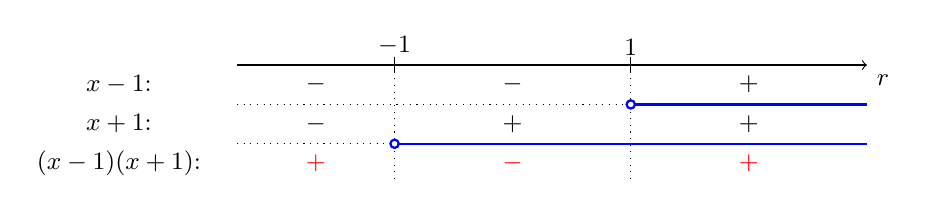
\begin{tikzpicture}[font=\small,x=10mm, y=10mm]

\draw[->] (0,0) -- (8,0) node [below right] () {$r$};

\foreach \x in {2,5}{
\draw(\x,3pt)--(\x,-3pt);
\begin{scope}[dotted]
\draw (\x,0) -- (\x,-1.5);
\draw (0,-.5) -- (5,-.5);
\draw (0,-1) -- (2,-1);
\end{scope}}

\node[above]  at (2,0) {$-1$};
\node[above]  at (5,0) {$1$};

\begin{scope}[blue,thick]
\draw (5,-.5) -- (8,-.5);
\draw (2,-1) -- (8,-1);

\draw[fill=white] (5,-.5)circle (1.5pt);
\draw[fill=white] (2,-1)circle (1.5pt);
\end{scope}

\foreach \x in {-1.5}{
\node  at (\x,-.25) {$x-1$:};
\node  at (\x,-.75) {$x+1$:};
\node  at (\x,-1.25) {$(x-1)(x+1)$:};
}
\foreach \z in {1,3.5}{
\node  at (\z,-.25) {$-$};
}
\foreach \zi in {3.5, 6.5}{
\node  at (\zi,-.75) {$+$};
}

\node  at (6.5,-.25) {$+$};
\node  at (1,-.75) {$-$};

\begin{scope}[red]
\foreach \zii in {1, 6.5}{
\node  at (\zii,-1.25) {$+$};
}
\node  at (3.5,-1.25) {$-$};
\end{scope}
\end{tikzpicture}

% \end{center}
% \item Semplifichiamo i radicandi 
%  \(\sqrt[3]{\dfrac{x^2}{(x-1)^2}}:\sqrt[4]{(x-1)\cdot (x+1)}\)
% \item Riduciamo allo stesso indice: il \(\mcm\) degli indici è \(12\), 
% quindi:
% 
% \(\sqrt[12]{\left[\frac{x^2}{(x-1)^2}\right]^4}:\sqrt[12]{(x-1)^3 (x+1)^3}
% \Rightarrow 
% \sqrt[12]{\frac{x^8}{(x-1)^8}\cdot \frac 1{(x-1)^3 (x+1)^3}}=
% \sqrt[12]{\frac{x^8}{(x-1)^{11}(x+1)^3}}\).
% \end{enumeratea}
% \end{esempio}

